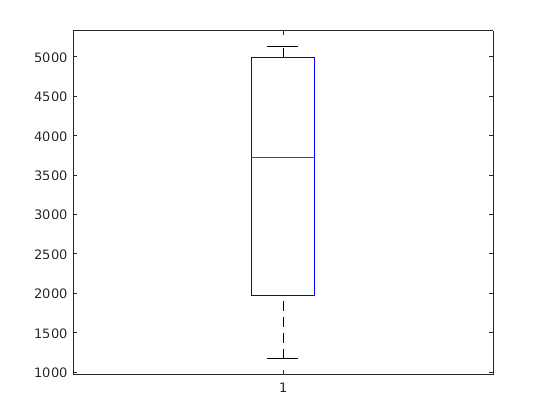
\includegraphics{Graphik/income1}
\begin{enumerate}
	\item Die Figur (..) zeigt das Boxplot-Diagramm von income1 
	\begin{itemize}
		\item Daten für ein Diagram müssen in einer Spalte liegen
		\item Daten müssen nicht sortiert sein
		\item Min- und Max-Werte sind jeweils durch den oberen bzw unteren Querstrich dargestllt
		\item Der Durschnitt (mean) ist der mittlere Abstand der äußeren  Striche
		\item Der Median (also das 50.Perzentil) wird durch den roten Querstricht innerhalb der Box dargestellt
		\item Q1 und Q3 sind jeweils Anfang bzw Ende der blauen Box
		\item um ein Boxplot-Diagram zu erstellen folgt man folgenden Schritten:
		\begin{enumerate}
			\item figure(1)
			\item boxplot(income1)
		\end{enumerate}
	\end{itemize}
	\item Die Figur (..) zeigt den Vergleich von income1 und income2
	\begin{itemize}
		\item Da sich die Anzahl der Datensätze verändert hat ist die Box (leicht) verschoben (also Q1 und Q3)
		\item aus den gleichen Gründen hat sich auch der Median verschoben 
		\item das rote Kreuz ist ein Ausreißer der sehr weit von dem Rest abweicht
	\end{itemize}
	\item Um vor Ausreißern gefeit zu sein empfiehlt sich die Betrachtung des Medians bei dichten Wertemengen
\end{enumerate}
